\newcommand{\psionDescription}{
\section{Psion}
\epigraph{\textit{
    "Resist all you like. I have ways of making you think." } }{ Dechares, Dwarven inquisitor }

    The psion learns the Way, a philosophy of mental
    discipline, to become master of his will, or innate mental
    power. Most aspiring psions seek out an instructor, a
    master of the Way. Most Athasian cities contain psionic
    academies where students receive instructions in
    exchange for money or loyal service.\\
    \\
    See \nref{tlttree:psion} for more information.
}

\newcommand{\psionTree}{
    \newpage
    \subsection{Psion Talent Tree}
    \label{tlttree:psion}

    \textbf{Class Skills:} Cool, Psionics, Perception, Vigilance, Discipline, Resilience
    \newline

    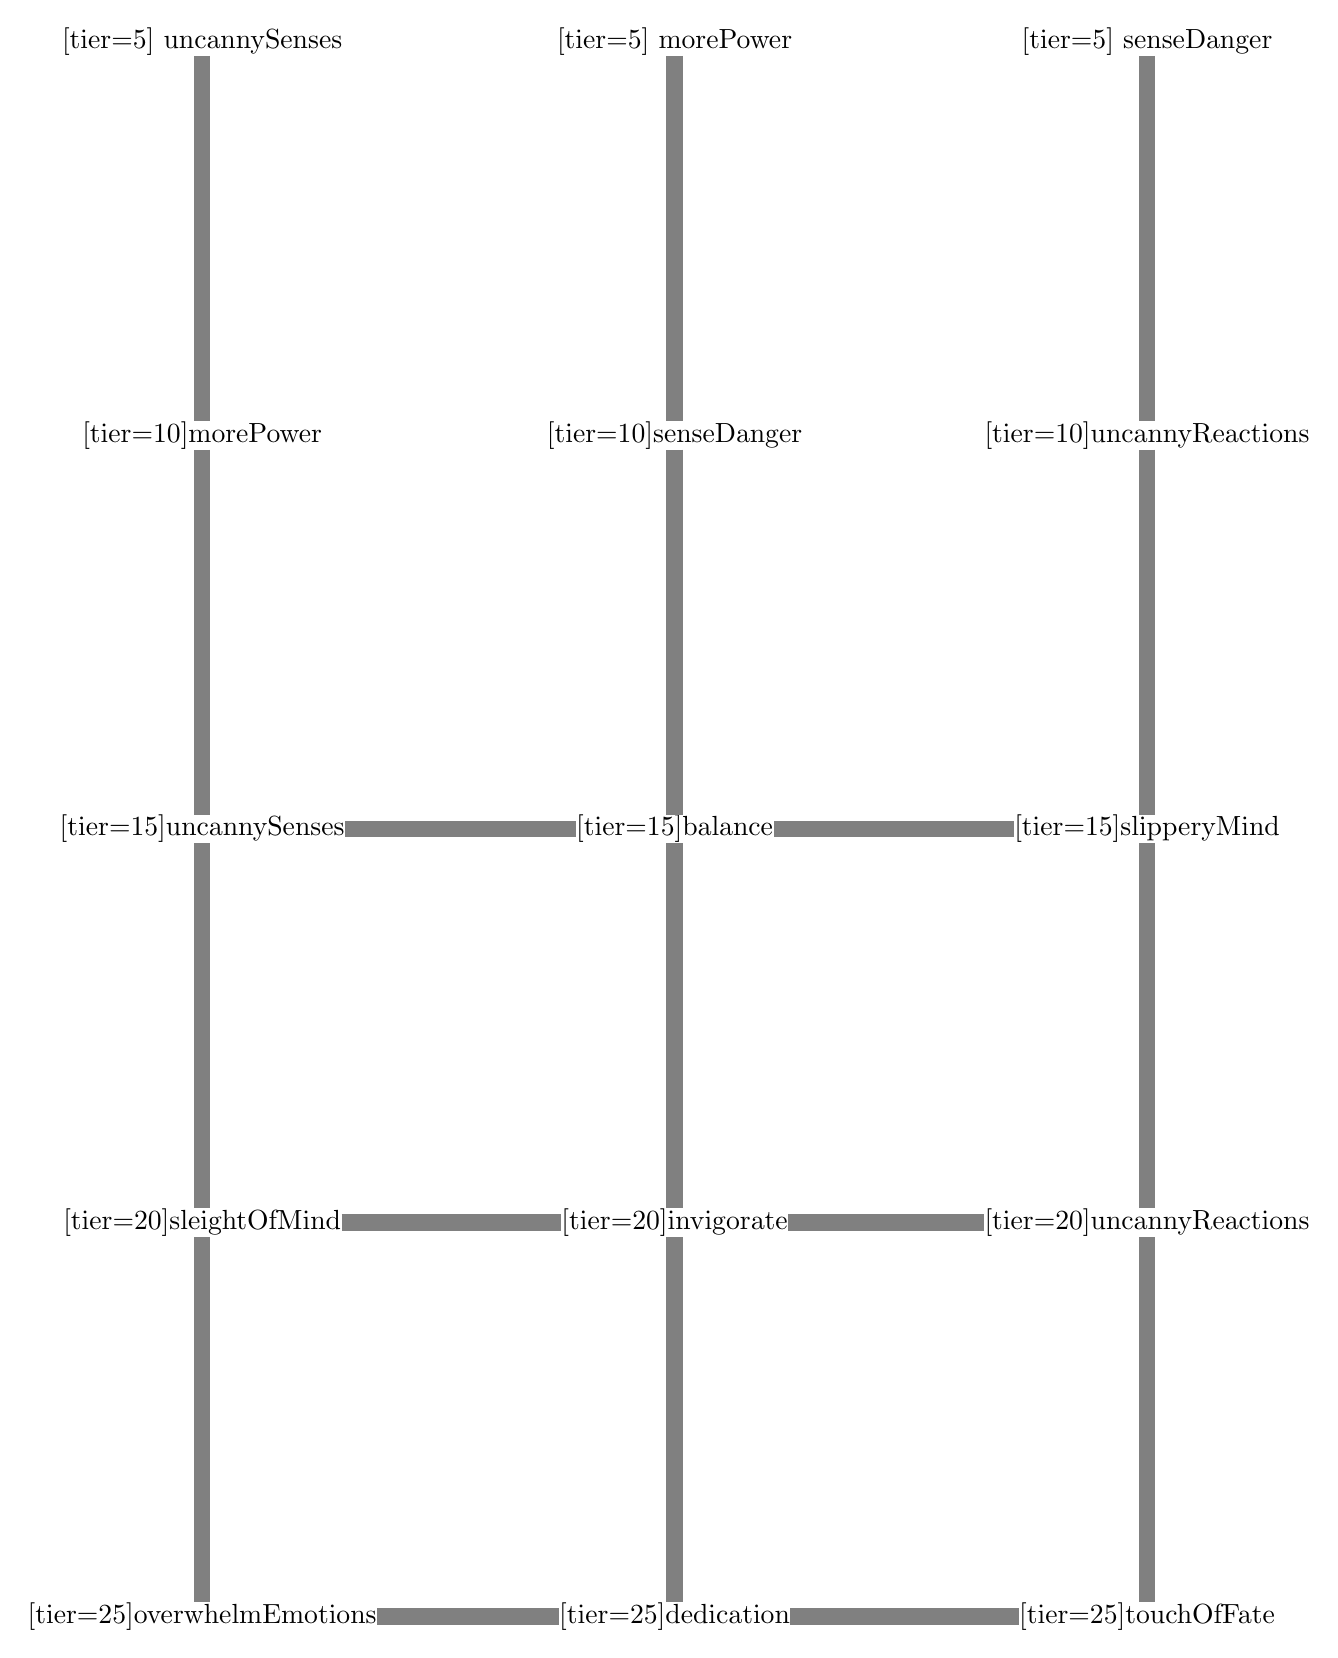
\begin{tikzpicture}
        \draw ( 0,  0) node(aa)[inner sep=0]{\TalentBox[tier=5] {uncannySenses}}
              ( 6,  0) node(ab)[inner sep=0]{\TalentBox[tier=5] {morePower}}
              (12,  0) node(ac)[inner sep=0]{\TalentBox[tier=5] {senseDanger}}
              ( 0, -5) node(ba)[inner sep=0]{\TalentBox[tier=10]{morePower}}
              ( 6, -5) node(bb)[inner sep=0]{\TalentBox[tier=10]{senseDanger}}
              (12, -5) node(bc)[inner sep=0]{\TalentBox[tier=10]{uncannyReactions}}
              ( 0,-10) node(ca)[inner sep=0]{\TalentBox[tier=15]{uncannySenses}}
              ( 6,-10) node(cb)[inner sep=0]{\TalentBox[tier=15]{balance}}
              (12,-10) node(cc)[inner sep=0]{\TalentBox[tier=15]{slipperyMind}}
              ( 0,-15) node(da)[inner sep=0]{\TalentBox[tier=20]{sleightOfMind}}
              ( 6,-15) node(db)[inner sep=0]{\TalentBox[tier=20]{invigorate}}
              (12,-15) node(dc)[inner sep=0]{\TalentBox[tier=20]{uncannyReactions}}
              ( 0,-20) node(ea)[inner sep=0]{\TalentBox[tier=25]{overwhelmEmotions}}
              ( 6,-20) node(eb)[inner sep=0]{\TalentBox[tier=25]{dedication}}
              (12,-20) node(ec)[inner sep=0]{\TalentBox[tier=25]{touchOfFate}}
        ;

        \tikzstyle{bar}=[gray,-,>=stealth, line width=6pt]

        \draw [bar] (aa) to (ba);
        \draw [bar] (ab) to (bb);
        \draw [bar] (ac) to (bc);

        \draw [bar] (ba) to (ca);
        \draw [bar] (bb) to (cb);
        \draw [bar] (bc) to (cc);

        \draw [bar] (ca) to (da);
        \draw [bar] (cb) to (db);
        \draw [bar] (cc) to (dc);

        \draw [bar] (da) to (ea);
        \draw [bar] (db) to (eb);
        \draw [bar] (dc) to (ec);

        \draw [bar] (ca) to (cb);
        \draw [bar] (cc) to (cb);

        \draw [bar] (da) to (db);
        \draw [bar] (dc) to (db);

        \draw [bar] (ea) to (eb);
        \draw [bar] (ec) to (eb);
    \end{tikzpicture}
}
